%\documentclass[sigconf, review, anonymous, screen]{acmart}
\documentclass[10pt]{article}
\usepackage[top=3cm, bottom=3cm, left=3cm, right=3cm]{geometry}
% The preceding line is only needed to identify funding in the first footnote. If that is unneeded, please comment it out.
\usepackage{kotex}
\usepackage{amsmath,amssymb,amsfonts}
\usepackage{algorithmic}
\usepackage{graphicx}
\usepackage{textcomp}
\usepackage{xcolor}

\usepackage[ruled,vlined,linesnumbered]{algorithm2e}

\usepackage{booktabs} % For formal tables
\usepackage{subcaption} % for subfigures

\usepackage{fancyhdr}
\usepackage{tabularx}
\usepackage{multirow}
\usepackage{multicol}
\usepackage{mdwlist}
\usepackage{indentfirst}
\usepackage{physics}
\usepackage{xspace}
\usepackage{tablefootnote}
\usepackage[bottom]{footmisc}
\usepackage{footnote}
\usepackage{hyperref}
\usepackage{makecell}
\usepackage{subcaption}
\usepackage[bottom]{footmisc}
\usepackage{balance}
\xspaceaddexceptions{]\}}

% Definitions
\newcommand{\blue}[1]{{\color{blue} #1}}
\newcommand{\red}[1]{{\color{red} #1}}
\newcommand{\orange}[1]{{\color{orange} #1}}

% math symbol definitions
\newcommand{\mat}[1]{\mathbf{#1}}
\newcommand{\ve}[1]{\mathbf{#1}}
\newcommand{\set}[1]{\mathbb{#1}}
\newcommand{\seq}[2]{\mathcal{#1}^{#2}}

% paper-dependent definitions
\newcommand{\User}{\set{U}}
\newcommand{\Item}{\set{I}}
\newcommand{\Su}{\seq{S}{u}}

% pre-defined names
\newcommand{\dqnname}{\textsc{DQN}}
\newcommand{\dqn}{\dqnname\space}

\newcommand{\sdqnname}{\textsc{S-DQN}}
\newcommand{\sdqn}{\sdqnname\space}

\newcommand{\sadqnname}{\textsc{SA-DQN}}
\newcommand{\sadqn}{\sadqnname\space}

\newcommand{\sapdqnname}{\textsc{SA-DQN+}}
\newcommand{\sapdqn}{\sapdqnname\space}


%\setlength{\belowcaptionskip}{-0.3cm}
\begin{document}
\title{[Super Mario RL] 대규모 데이터분석 특강 - 프로젝트 보고서}

\author{
구본헌 \& 김정훈\\
Department of Computer Science and Engineering\\
Seoul National University\\
\texttt{\{darkgs, rlawjdgns434\}@snu.ac.kr}\\
\texttt{2019-\{36050,29394\}}\\
}

\renewcommand{\baselinestretch}{1.25}

\maketitle
% Sec 0. Abstract
\begin{abstract}
본 프로젝트 보고서는 2019년도 봄학기 대규모 데이터분석 특강 과목의 조별 프로젝트의 내용을 담고 있다.
우리는 슈퍼 마리오 브라더스 게임을 강화학습을 통해 높은 점수로 플레이하는 모델을 개발하는 것을 목표로 한다.
이를 위해 우리는 먼저 게임 플레이를 대상으로 하는 강화학습 기법들에 대해 발표된 논문을 조사하여, 우리 모델을 구성할 때 고려할 점과 아이디어를 얻기위한 기반으로 삼았다.
또한, 슈퍼 마리오 브라더스 게임을 분석하여 강화학습 모델에 어떻게 적용할지 알아보고 구체적인 개발환경을 조사한 후 일정을 수립하였다.
\end{abstract}

%\keywords{
%Reinforcement Learning; 강화 학습
%}


% Sec 1. Introduction
\section{Introduction}
\label{sec:intro}
본 대규모 데이터분석 특강 프로젝트에서 우리는 슈퍼 마리오 브라더스 게임을 강화학습을통해 컴퓨터가 학습하고 최종적으로 높은 점수로 스테이지를 클리어 하는 것을 목표로 한다.

슈퍼 마리오 브라더스에서 사용 가능한 동작은 총 6 가지로 구성되어 있으나 서로 다른 키를 조합하여 입력하는 것이 가능하므로 실제로 사용 가능한 동작은 총 16개로 구성되어 있다. 해당 게임은 agent인 마리오가 목적지에 도달하거나, 적에게 부딪히거나, 제한 시간 내에 목적지에 도달하지 못하면 stage가 끝남으로써 episodic한 요소를 가지고 있다. 

따라서 해당 게임을 강화학습을 통해 클리어하기 위해 실제 인간에게 주어지는 것처럼 현재 화면을 입력 값으로 받고 이를 통해 최적의 동작(action)을 찾아내는 모델인 convolutional neural network (CNN)을 구축하는 것을 기반으로 다양한 시도를 할 것이다.

프로젝트 기간내에 효율적으로 시간을 분배해 최적의 결과를 도출하기 위해 각 구성원의 역할을 개발환경 세팅, 기존 방법 학습, 새로운 방법 연구, 제안 방법 개발과 같은 방식으로 세분화한다.

해당 프로젝트 제안서의 구성은 다음과 같다. 
2 장에서는 본 프로젝트에서 풀려고 하는 슈퍼 마리오 브라더스 게임을 학습하고 목표를 달성하기 위해 도움이 될만한 기존 논문의 메인 아이디어를 간략히 설명하고 어떻게 프로젝트 구현에 사용될 수 있을지에 대해 설명한다. 
또한 논문의 메소드를 본 프로젝트에서 사용함에 있어 제약사항 혹은 문제가 될 여지가 있다면 이러한 부분에 대해 서술한다. 
3 장에서는 슈퍼 마리오 브라더스 게임에 대해 간략히 설명하고 강화학습을 진행하는데 필요한 state, action, 그리고 reward이 게임에서 어떻게 구성되어 있는지에 대해 설명한다. 
4 장에서는 본 프로젝트에서 사용할 라이브러리에 대한 설명과 각 구성원의 개발 일정에 따른 역할에 대해 설명한다. 
마지막으로 5 장에서는 해당 제안서에서 설명한 부분들에 대해 정리한 뒤 본 프로젝트 제안서를 마무리하는 것으로 구성되어 있다.

\section{Paper Survey}
본 절에서 우리는 게임에 적용된 강화학습 기법을 소개한 논문을 조사한 결과를 소개한다.
먼저 아타리 게임을 통한 강화학습 연구의 시초인 Deep Q-Networks (DQN)을 하위 섹션~\ref{sec:survey:DQN}에서 다루며, 이를 발전시킨 Dueling Network를 다룬 논문을 하위 섹션~\ref{sec:survey:DuelNet}에서 소개한다.
Policy gradient 방법으로 넘어가서, deterministic policy gradient (DPG)를 하위 섹션~\ref{sec:survey:DPG}에서 소개한 후,
이에 actor-critic 개념을 입혀 개량한 deep deterministic policy gradient (DDPG)를 하위 섹션~\ref{sec:survey:DDPG}에서 다룬다.
GPU 가속을 통한 병렬처리 컴퓨팅 환경을 효율적으로 이용하도록 설계된 Asynchronous Actor-Critic (A3c)의 컨셉에 대해 하위 섹션~\ref{sec:survey:A3C}에서 알아본다.
마지막으로 action의 선택과 평가에 쓰이는 weight set을 분리하여 value값이 과평가되는 것을 방지하는 Double Q-learning에 대해 하위 섹션~\ref{sec:survey:DoubleQ}에서 소개한다.
\label{sec:survey}
\subsection{Playing Atari with Deep Reinforcement Learning}
\label{sec:survey:DQN}
해당 논문~\cite{DQN}은 딥러닝 알고리즘으로 action-value function의 Q 값을 예측하는 기법인 Deep Q-Networks (DQN)을 제시하였다. 
논문 제목에서도 볼 수 있듯이 새로운 메소드를 Atari 2600이라는 고전 게임 모음 중 대표적인 7 개의 게임을 통해 그 성능을 확인하였다. 
Atari 2600 게임은 action에 대한 transition 확률과 reward가 명시적으로 주어지지 않은 model-free 문제이다.

해당 논문에서 볼 수 있는 특이한 점은 입력 값으로 게임의 이미지 전체를 받는다는 점인데, 기존 강화 학습에서 state를 정의할 때 게임 이미지의 각 픽셀을 하나의 state로 정의하여 에이전트에게 전달하는 것과는 다르면서 색다른 방식이다. 
따라서 게임의 이미지 화면을 입력 값으로 받으면 딥러닝 알고리즘에서 이미지 처리에 탁월한 Convolutional Neural Networks (CNN)을 통해 계산된 Q값을 에이전트에게 전달하고 해당 값을 기반으로 최적의 action을 실행하여 게임을 진행하는 방식으로 구성되어 있다. 

여기서 눈 여겨 봐야할 점은 Q값을 구하기 위해 CNN을 사용하였다는 것인데, 이는 기본적으로 사용되는 value iteration 알고리즘과 같은 문제점을 해결한다. 
Value iteration 알고리즘은 논문과 같은 환경인 transition 확률과 reward가 명시적으로 주어지지 않은 조건에서는 동작하기 어려운 점이 있다. 
그러나 해당 논문에서 사용하는 Q-Networks는 이러한 model-free 문제에서 neural network value function approximator를 통한 샘플링을 통해 Q값을 구한다. 
따라서 학습을 할 때 Q-network에서는 손실 함수를 최소화하면서 그 성능을 높인다. 

논문에서 보여준 이러한 방식은 우리가 풀려는 슈퍼마리오 게임에서의 환경과 비슷한 점이 많기 때문에 논문에서 제시한 DQN 알고리즘을 사용할 예정이다. 
슈퍼마리오 게임 또한 Atari 게임과 같이 게임 화면이 state로 주어지고 finite한 게임 내에서 게임이 한 에피소드를 끝내기 위한 조건도 유사하기 때문에 논문에서 제시한 알고리즘을 사용한다면 높은 성능을 보일 것이라 판단한다. 

그러나 해당 논문에서 제시한 DQN은 Q-learning 값을 업데이트 하는 과정에 있어서 max 연산자를 사용하기 때문에 Q-value를 실제보다 높게 평가하고 그 결과 학습이 느려지는 경향이 있다. 
따라서 실험에 사용한 Atari 게임은 우리가 풀려는 슈퍼마리오 게임보다 상대적으로 크기가 작고 간단하기 때문에 슈퍼마리오 게임과 같이 더 크고 복잡한 조건에서도 과연 학습이 느려질 수 있다는 것에 대한 제약사항이 존재할 가능성이 있다. 


\subsection{Dueling Network Architectures for Deep Reinforcement Learning}
DQN알고리즘이 큰 성과를 이루며 deep Q learning에 대한 발전 속도는 굉장히 빨라졌는데, 해당 논문 또한 DQN 알고리즘을 기반한 새로운 네트워크 구조를 개발한 논문이다. 
기존의 DQN은 특정 지점에서의 Q function을 추정(estimate)하기 위하여 모든 state와 action의 값을 모두 평가해야 한다. 
그러나 대부분의 경우에는 state의 가치가 중요하고 action으로 인한 가치의 변화가 극명한 경우는 많지 않다. 
따라서 해당 논문은 Figure~\ref{fig:dueling_network}과 같이 새로운 DQN 구조(dueling network)를 제안했다.

\begin{figure}[h]
\begin{center}
\begin{tabular}{c}
     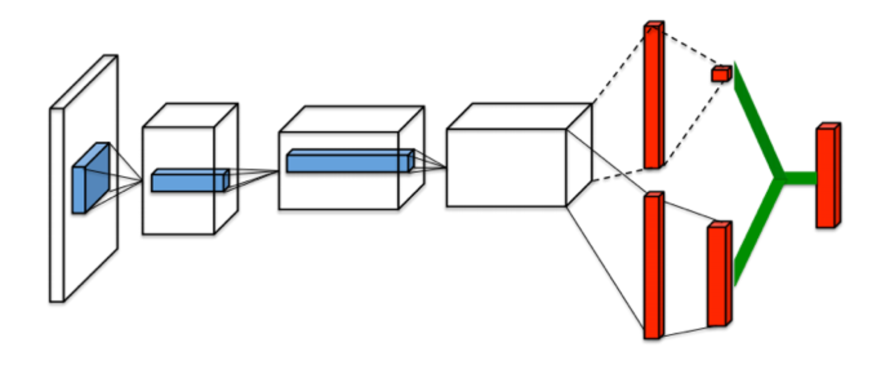
\includegraphics[width=0.45\textwidth]{FIG/DuelingNetwork.png} \\
\end{tabular}
\caption{
	Dueling Network의 구조.
}
\label{fig:dueling_network}
\end{center}
\end{figure}

앞서 말한 것처럼, 해당 논문에서의 네트워크 구조는 새로운 DQN 구조를 가지고 있는데 Q 값의 정의로부터 유도되는 한 가지 수식에서 아이디어를 얻어 탄생했다. 
해당 수식은 아래와 같다. 
\begin{align*}
	Q(s,a) = V(s) + A(s,a) \\
\end{align*}
Q 값의 의미는 현재 상태에서 행동을 취할 때 얻을 수 있는 보상의 합을 말한다. 
해당 논문에서는 이 값을 두가지로 분리하였는데 Value function(V)와 Advantage function(A)이다. 
V 값은 현재 상태에서 최선의 행동을 취했을 때 얻을 수 있는 보상의 합이고, A는 최선인 행동과 다른 행동들 사이의 보상의 차를 의미한다. 
이러한 구조를 자세히 보면 Q 값을 추론하는 것을 두 가지로 분리해서 생각한 것인데, 현재 상태가 좋은지 나쁜지를 V 값으로 추론하고 그 중에서 어떤 행동을 고를지를 A 값을 이용하여 추론한다. 
따라서 V 값은 바이어스 같은 역할을 하고 V를 중심으로 좋고 나쁨을 A 값을 이용하여 추론하게 되는 것이다. 

Dueling Network 또한 DQN과 마찬가지로 게임 이미지를 입력 값으로 받아 Q 값을 추정(estimate)한다. 
해당 논문에서 제시한 알고리즘은 Atari 게임에서 DQN을 더불어 다른 메소드보다 높은 성능을 보였다.

앞서 말한 것과 같이 우리의 프로젝트 또한 Atari 게임과 비슷한 환경을 가지고 있기 때문에 해당 알고리즘을 사용하여 성능을 높일 수 있을 거라 판단한다. 
또한 논문에서는 해당 알고리즘은 기존에 존재하는 여러 알고리즘(DQN, SARSA)에서도 사용될 수 있다고 설명한다. 
따라서 프로젝트에서 DQN으로 시도를 할 것을 염두하고 있기 때문에 DQN 혹은 DDQN을 사용할 경우 해당 알고리즘을 추가하여 손쉽게 성능을 높이기 위한 추가적인 시도를 할 것이다.

\subsection{Deterministic Policy Gradient Algorithms}
\label{sec:survey:DPG}
앞서 살펴본 DQN과 같은 방법은 value function을 학습하는 방식이기 때문에 만약 value가 살짝 바뀌어도 policy가 같이 변하여 학습 과정이 불안정하게 되고 수렴이 불안정해지는 단점이 있다. 
따라서 policy 자체를 예측을 하면 되지 않을까라는 개념으로 탄생한 것이 policy gradient 알고리즘이다. 

policy gradient 알고리즘은 expected reward를 policy의 파라미터에 대한 함수로 모델링하고 이 reward를 최대화하는 policy를 gradient ascent 기법을 사용해서 찾는 기법이다.
해당 기법은 policy의 변화를 통해 더 나은 policy를 찾아가는 방식으로 구성되어 있다. 
최적의 policy는 stochastic한 성질을 가지는 경우가 많기 때문에 stochastic policy gradient 방식을 선호하였는데 해당 논문을 통해 deterministic policy gradient가 high-dimensional task에서 보다 빠르게 동작한다는 것을 증명하였다. 

해당 논문에서는 octopus arm 실험을 통해 성능을 측정하였는데 해당 실험을 사용한 이유는 high dimensional task에서의 성능을 확인하기 위함이다 (Figure~\ref{fig:dueling_network} 참조).
해당 실험에서 목표는 6 개의 구획으로 구성된 다리를 움직여 오렌지 색상의 음식을 검은색 입으로 전달하여 보상을 얻는 것이다.
환경에서는 50 개의 continuous 한 state가 존재하며 각 구획에는 회전 및 이동할 수 있는 muscle이 존재해 한 구획당 총 20 가지의 동작이 가능하다. 
이러한 실험에서 높은 성능을 보였고 high dimensional 한 task에서는 deterministic policy gradient 알고리즘이 stochastic의 경우보다 성능이 좋다는 것을 확인하였다.

\begin{figure}[h]
\begin{center}
\begin{tabular}{c}
     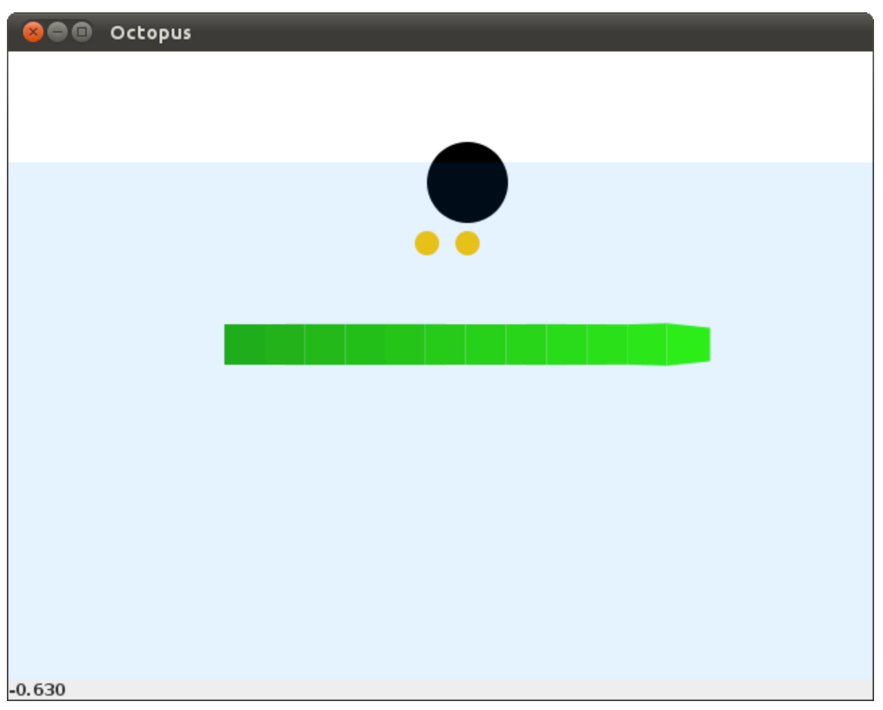
\includegraphics[width=0.45\textwidth]{FIG/OctopusArm.png} \\
\end{tabular}
\caption{
	Octopus Arm Environment.
}
\label{fig:octopus_arm}
\end{center}
\end{figure}

policy gradient 알고리즘은 continuous 한 action space 상황에서 자주 사용되는데 본 프로젝트에서 실험하는 슈퍼 마리오 브라더스는 discrete 한 action space 상황이기 때문에 deterministic policy gradient 알고리즘을 바로 적용할 수는 없다. 
그러나 해당 논문을 통해 우리 모델의 성능을 높이기 위해 policy gradient를 적용한다는 아이디어를 참고할 수 있기에 해당 논문을 서베이 목록에 추가하였다.

\subsection{Deep Deterministic Policy Gradient}
Deep Deterministic Policy Gradient (DDPG)는 state와 action을 입력으로 받아 각 action에 대한 value값을 산출해내는 Q-function을 학습시키는 방법이다.
DDPG의 핵심 동작은 아래와 같은 식으로 나타낼 수 있다.
\begin{align*}
	a^*(s) &= arg \underset{a}{max} Q^*(s,a) \\
\end{align*}
%\begin{align*}
%	h_t &= f(h_{t-1},x_t;W,b) \\
%		&= \tanh{(W_{hh}h_{t-1}+W_{hx}x_t+b_h)} \\
%		&= \tanh{(W_{h}[h_{t-1},x_t]+b_h)}
%\end{align*}
여기서 Q-function Q 는 action a와 state s를 입력으로 받아 value를 판별해주므로 최대 value를 가지는 action을 선택하면 최적화된 policy를 구할 수 있다.

DDPG는 다음과 같은 특징을 가지고 있다.
\begin{itemize}
	\item off-policy 방법
	\item continuous action space에서만 동작하는 방법
	\item 병렬화된 학습 방법을 제공하지 않음
\end{itemize}
본 프로젝트에서 학습하기로 한 게임인 슈퍼 마리오 브라더스는 discrete한 action space를 가지므로 DDPG 알고리즘을 바로 적용할 수는 없다.
하지만 DDPG에서 학습을 돕기 위한 주요 아이디어를 차용하여 우리 프로젝트에 적용해 볼 수 있다.

\paragraph{\textbf{Replay Buffer:}}
음냐
\paragraph{\textbf{Target Network:}}
음냐

\subsection{Asynchronous Actor-Critic}
Volodymyr Mnih, et. al. 이 제안한 Asynchronous Actor-Critic (A3C)~\cite{A3C}는 게임 플레이를 위한 강화학습에 널리 쓰이는 방법이다.


\subsection{Double Q-learning}
...


\section{Preliminaries}
\label{sec:preliminaries}
본 장에서는 이번 프로젝트의 타겟 게임인 슈퍼 마리오 브라더스 게임을 하위 섹션~\ref{sec:method:smb}에서 소개한다.

\subsection{슈퍼 마리오 브라더스}
\label{sec:method:smb}

\begin{figure}[h]
\begin{center}
\begin{tabular}{c}
     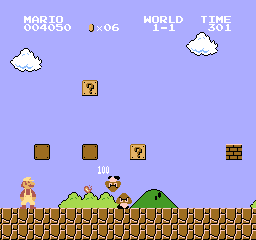
\includegraphics[width=0.45\textwidth]{FIG/SuperMarioBros.png} \\
\end{tabular}
\caption{
	슈퍼 마리오 브라더스의 게임 화면.
}
\label{fig:mario_title}
\end{center}
\end{figure}

슈퍼 마리오 브라더스는 닌텐도 초기의 액션 게임으로 1985년 9월 13일 NES (Nintendo Entertainment System) 전용 게임으로 출시 되었다.
Figure~\ref{fig:mario_title}은 이 게임의 플레이 화면이다.
당시 출시된 다른 게임들과 비교하여 우수한 조작감과 완성도 높은 미술로 크게 흥행하였으며 현재 2019년도 까지고 지속적으로 후속작이 출시되고 있다.
간단한 조작으로도 자유도 높은 플레이가 가능하여 강화학습의 목표로 삼기에 적합하여 이번 프로젝트의 대상으로 선택하였다.
슈퍼 마리오 브라더스는 총 8개의 world 와 각 world 당 4개의 stage로 구성되어 있다.
각 world 별로 특징있는 컨셉을 (물의 나라, 얼음의 나라, 등) 가지고 디자인 되어 배경 및 등장하는 적 케릭터가 차이가 있다.
또한 world 및 stage 수가 증가할 수록 난이도가 올라가는 경향을 가진다.

\begin{table}[h]
\centering
	\caption {
		슈퍼 마리오 브라더스에서 가능한 키 입력. 서로 다른 키를 조합하여 입력하는 것이 가능하다.
	}
	\label{tab:mario:key}
\begin{tabular}{ll}
\toprule
키     & \multicolumn{1}{c}{동작 설명} \\
\midrule
up    & 특수한 상황(넝쿨, 파이프)에서 마리오를 위로 이동 \\
left  & 마리오를 왼쪽으로 이동 \\
down  & 특수한 상황(넝쿨, 파이프)에서 마리오를 아래로 이동 \\
right & 마리오를 오른쪽으로 이동 \\
A     & 가속 또는 불꽃 공격(슈퍼 마리오만 해당)\\
B     & 점프 \\
\bottomrule
\end{tabular}
\end{table}

Table~\ref{tab:mario:key} 에서 슈퍼 마리오 브라더스 게임에서 가능한 모든 키 입력을 소개한다.
모든 입력은 중복하여 입력하여 마리오가 다른 동작을 하게 할 수 있다.
예를 들면 right 키와 B 키를 동시에 입력하면 마리오가 오른쪽으로 나아가며 점프한다.
하지만 경우에 따라 right 키와 left 키를 동시에 누른 경우 처럼 상보적인 두 가지 키를 조합하는 경우 무의미한 동작을 나타낼 수도 있다.
슈퍼 마리오 브라더스 게임에서 유의미한 키조합을 고려할 경우 가능한 Action의 경우의 수는 16가지 이다.

슈퍼 마리오 브라더스에서 목적지인 깃발로 이동하면 한 stage가 종료된다.
그 외에는 적에게 부딧치거나, 함정에 빠진 경우, 그리고 제한 시간이 지난 경우 stage가 종료되며 처음부터 다시 시작하게 된다.
이 게임의 목적은 보다 많은 점수를 얻으면서 깃발에 도달하여 stage를 완료하는 것이다.
stage 내부에서 점수를 얻는 방법은 아래와 같다.
\begin{itemize}
	\item \textbf{깃발 도달시 남은 시간:}
		제한 시간 이내에 깃발에 도달한 경우 남은 시간 (초 단위)당 100점 획득.
	\item \textbf{동전을 획득:}
		stage내에서 벽돌, 물음표 블록, 그리고 동전 아이템을 통해 동전에 닿으면 100점 획득.
	\item \textbf{버섯, 꽃을 획득:}
		stage내의 물음표 블록에서 버섯 또는 꽃이 나왔을 때 닿으면 100점 획득.
	\item \textbf{적을 처치:}
		적을 처치시 기본적으로 100점 획득하며 연속된 처치를 할 경우 매번 2배의 추가 점수 획득.
\end{itemize}

이 게임에서 stage별로 목적지에 도달하지 못하고 종료된 경우 다시 도전할 기회를 부여하는 데 이 횟수는 마리오의 남은 생명으로 결정된다.
게임내에서 녹색 버섯을 획득하거나 동전을 100개 모은 경우 추가로 보너스 생명을 1개 얻게 된다.
강화학습을 위한 환경에서는 학습을 시키기 위해 stage를 수 많이 반복하여야 하여 이러한 재도전 횟수를 제한하는 것을 해제한 상태에서 학습시키게 된다.
하지만 실제 플레이어가 게임을 한다고 가정할 때 이러한 생명을 관리하는 것은 게임을 끝까지 완수하기 위한 중요한 요소이다.


\section{Proposed Method}
\label{sec:method}
해당 장에서는 이번 프로젝트를 진행하면서 사용한 메소드에 대해 설명한다.
프로젝트의 주제인 슈퍼 마리오 게임 특성상 게임 화면을 통해 내용이 전개된다. 
따라서 우리는 \ref{sec:survey:DQN}에서 설명한 DQN 메소드를 기본으로 사용한다.
기존 발표된 기법 중 하나인 Deep Q-Network(DQN) 메소드에 추가적인 화면 분할을 통해 여러 구역을 학습하는 Split DQN을 설명하고, 최종적으로 Split DQN에 Attention 개념을 추가한 Split Attention DQN 메소드에 대해 설명한다.

위에서 간략히 설명한 제안 메소드를 설명하기에 앞서 이 게임에서 강화학습에 필요한 state, action, 그리고 reward를 어떻게 얻어내는지에 대해 하위 섹션~\ref{sec:method:basis}에서 다룬다.
섹션~\ref{sec:method:idea}에서는 Split DQN과 Split Attention DQN에 대해 소개한다.

\subsection{강화학습 기본 요소 추출}
\label{sec:method:basis}
강화학습에서 현재 state는 이 후 action을 결정하는 데 중요한 요소이다.
실제 게임 플레이어와 공평한 조건에서 경쟁하기 위해 본 프로젝트에서 state를 화면에 표시되는 이미지를 사용하여 결정하기로 하였다.
Convolutaionl neural network (CNN)~\cite{CNN}은 이미지로 부터 학습 모델에 필요한 feature를 추출하여 의사 결정에 활용하는 널리 알려진 방법이다.
본 프로젝트에서 우리는 화면 이미지를 CNN을 통해 해석하여 게임 점수를 최대한 얻을 수 있는 action을 추론하는 모델을 만들고자 한다.

우리는 키 조합을 통해 action을 생성할 수 있는데 유의미한 조합만을 고려하면 Table~\ref{tab:mario:action}과 같은 16개의 action을 정의할 수 있다.
여기서 유의미한 조합이라 함은, 무의미한 조합을 제외한 키 조합을 의미한다.
슈퍼 마리오는 총 6개의 키를 가지고 있으므로 총 64개의 키 조합을 가지는 데, 이 중 left + right와 같이 서로 상반되는 동작을 동시에 지정하는 경우에는 게임 내부의 키 매핑에 의해 아무 행동을 하지 않게 된다.
이러한 무의미한 action의 경우 우리의 학습 모델에 혼동만 주기 때문에 미리 제외하였다.
%
\begin{table}[h]
	\caption {
		슈퍼 마리오 브라더스에서 가능한 키 입력 조합. 가능한 조합 중 유의미한 키 조합만을 선별하였다.
	}
	\label{tab:mario:action}
\centering	
\begin{tabular}{lcccccc}
\toprule
          & Left & Right & Up & Down & A & B \\
\midrule
Action 1  &      &       &    &      &   &   \\
Action 2  & *    &       &    &      &   &   \\
Action 3  &      & *     &    &      &   &   \\
Action 4  &      &       & *  &      &   &   \\
Action 5  &      &       &    & *    &   &   \\
Action 6  &      &       &    &      & * &   \\
Action 7  &      &       &    &      &   & * \\
Action 8  &      &       &    &      & * & * \\
Action 9  & *    &       &    &      & * &   \\
Action 10 & *    &       &    &      &   & * \\
Action 11 & *    &       &    &      & * & * \\
Action 12 &      & *     &    &      & * &   \\
Action 13 &      & *     &    &      &   & * \\
Action 14 &      & *     &    &      & * & * \\
Action 15 &      &       & *  &      &   & * \\
Action 16 &      &       &    & *    &   & * \\
\bottomrule
\end{tabular}
\end{table}
%
우리의 모델은 최종적으로 Figure~\ref{fig:overview}와 같이 현재 state에서 각 차원이 각 action에 대응되는 16차원의 vector를 산출하여 각 action의 적합성을 확률적으로 추론한다.
\begin{figure}[]
\begin{center}
\begin{tabular}{c}
     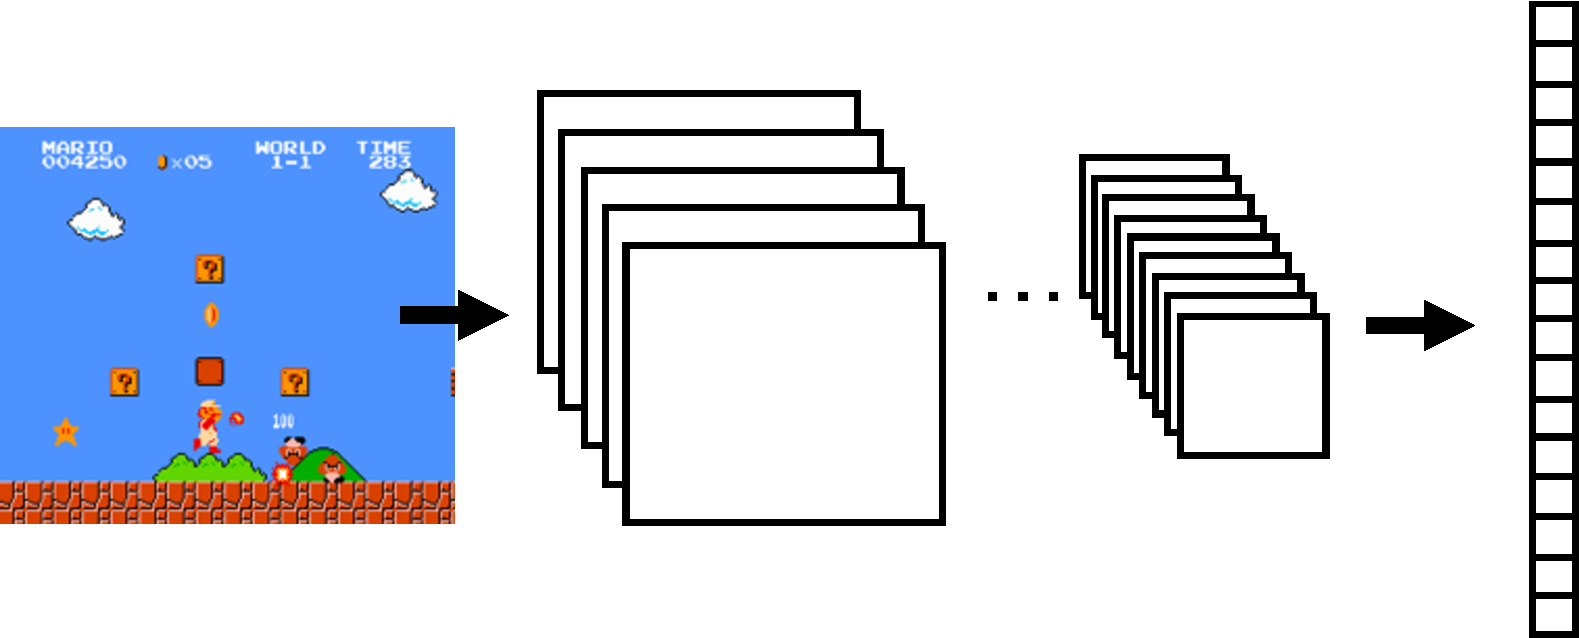
\includegraphics[width=0.4\textwidth]{FIG/overview.pdf} \\
\end{tabular}
\caption{
	게임 화면으로부터 action을 추론하기 위한 모델. CNN을 통해 게임화면을 해석하여 16차원의 action의 적합성을 추론한다.
}
\label{fig:overview}
\end{center}
\end{figure}

강화학습에서 모델은 현재 state에서 최종적으로 얻을 수 있는 reward를 극대화하는 action을 선택하도록 학습된다.
따라서 reward를 잘 설정해야 올바른 선택을 하도록 유도할 수 있다.
슈퍼 마리오 브라더스 게임에서 stage가 끝날 때 남은 시간당 50점을 획득하게 된다.
이는 다른 방법으로 얻는 점수보다 상당히 많은 양이다.
이번 프로젝트에서 해결하려는 것은 마리오를 가능한 빠른 시간 안에 목적지까지 도착하게 하는 것이다. 
따라서 획득 점수 위주로 reward를 설정하였을 때, 마리오가 빠른 시간안에 깃발로 도달하도록 유도할 수 있다.




이러한 방법 외에도 마리오의 이동 위치에 따라 추가적으로 reward를 제공하는 방법을 사용하였다. 
이러한 방법을 사용하는 이유는 마리오가 깃발에 가까워질수록 reward가 더 커지는 것을 인지하게 하려함이다. 
여러 시도 끝에 마리오가 목적지 방향인 오른쪽 방향으로 이동을 하였을 때 보상을 받고, 왼쪽 방향으로 이동을 하였을 때 패널티를 받는다면 마리오는 오른쪽 방향으로 이동하는 것이 보상을 받는다는 것을 인지하고, 왼쪽보다는 오른쪽으로 이동하려 할 것이다.
오른쪽 방향으로 이동함에 따라 reward를 제공하며 에이전트에게 골 라인으로 도달하는 가이드라인을 주는 효과를 볼 수 있다.
Reward를 제공하는 방식은 다음과 같다.
만약 마리오가 이전 위치보다 좌측으로 n만큼 이동하였다면 이는 목적지에서 더욱 멀어지는 방향으로 가고 있다 판단되어 -5만큼의 reward를 제공한다. 
반대로 만약 마리오가 이전 위치보다 우측으로 n만큼 이동하였다면 이는 목적지와 가까운 방향으로 이동하고 있고 목적지로 달성한다고 판단되어 +5만큼의 reward를 제공한다.
여기에 추가로 만약 마리오가 이전 위치에서 움직이지 않는다면 -1만큼의 reward를 제공함으로써 마리오를 목적지 방향으로 움직이려는 시도를 한다. 

위와 같은 reward를 제공하는 방법과 더불어 시간이 지남에 따라 패널티를 제공한다. 
한 스테이지가 시작되면 제한 시간이 존재한다. 
제한 시간안에 목적지에 도달하지 못하면 게임은 끝이 나는데, 제한 시간에 패널티를 제공하는 방식이다. 
시간이 1초가 지날 때마다 -1의 리워드를 제공하여 빠른 시간 안에 목적지에 도달할 수 있도록 구현하였다. 

% 삭제 해야하나영
또한, stage 중간에 코인, 아이템, 그리고 적을 처치해서 얻는 점수를 고려하면 중간중간의 imediate reward로 활용되어 마리오가 해당 동작을 하도록 하는 학습을 할 수 있다.
이와 같이, stage 내부의 획득 점수를 통해 reward를 주는 것은 올바른 게임 플레이를 학습하는 데 도움을 준다.

게임의 특성상 마리오를 큰 마리오, 나아가 슈퍼 마리오로 변신시키면 남은 stage를 진행함에 있어 크게 유리한 요소로 작용한다.
우리 모델이 슈퍼 마리오로 변신하는 것을 지향하고 변신이 풀리는 것을 지양하기 위해 상위 단계로 변신할 때 획득 점수이외의 부가적인 reward를 할당하고, 변신이 풀릴 경우 reward를 크게 감소시키도록 한다.

\subsection{DQN}
\label{sec:method:dqn}
DQN 설명

\subsection{Split DQN (\sdqnname)}
\label{sec:method:sdqn}
S-DQN 설명

\subsection{Split Attention DQN (\sadqnname)}
\label{sec:method:idea}
사람들이 슈퍼 마리오 브라더스를 실제로 플레이할 때, 사람들은 상황에 따라 화면의 일부분을 좀 더 집중해서 바라보게 된다.
예를 들면, 마리오가 공중에서 하강하고 있을 때는 마리오의 아래 쪽에 집중하여 바닥의 함정을 피하거나 적을 밟아 처치하도록 조작한다.
전반적으로, 전체 화면의 내용보다 마리오 주변에서 일어나고 있는 일에 집중하는 경향이 있다.

\begin{figure}[]
\begin{center}
\begin{tabular}{c}
     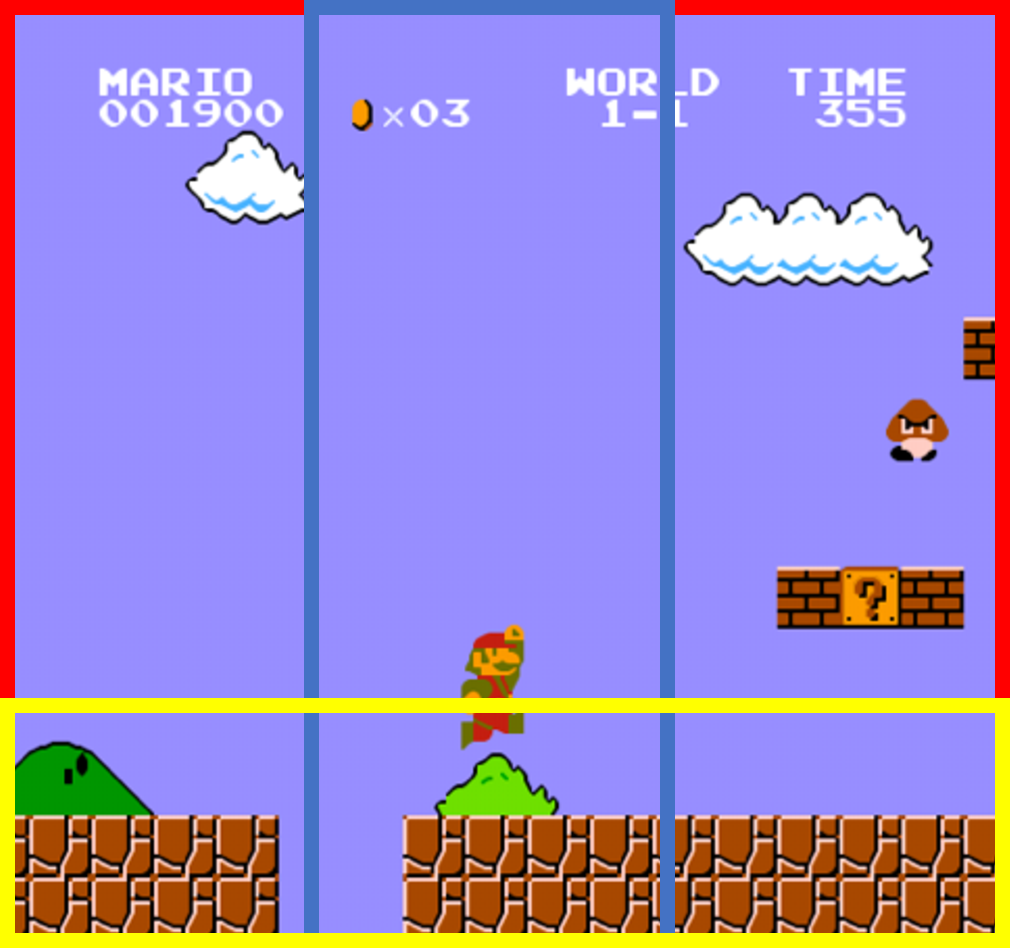
\includegraphics[width=0.4\textwidth]{FIG/split_screen.pdf} \\
\end{tabular}
\caption{
	화면 분할을 통해 여러 CNN 입력을 생성하는 예시. 전체 화면을 나타내는 빨간색, 마리오 주변을 나타내는 파란색, 그리고 바닥의 함정을 조심하기 위한 노란색 영역이 있다.
}
\label{fig:split_screen}
\end{center}
\end{figure}

이러한 게임의 특성을 고려하여 우리 모델도 여러 개의 CNN을 만들어 화면의 각 구역별로 따로 feature를 추출하기로 한다.
이렇게 추출한 feature의 중요도는 마리오의 상황에 따라 변화한다. 앞서 예와 같이 마리오가 공중에 있다면 마리오 주변에 좀 더 집중해야 한다.
만약 마리오의 달리기 속도가 빠른 상황이라면 좀 더 전체 화면부위를 고려하여 다음 action을 정해야한다.
또한 바닥의 함정에 빠지면 마리오가 즉사할 수 있으므로 아래 쪽 영역에 대한 주의도 늦출 수 없다.
우리 모델에서는 figure~\ref{fig:split_screen}과 같이 여러 구역으로 나눠 입력을 만든 후 각각의 CNN으로 생성된 feature를 마리오의 현재 상황에 따라 중요도를 계산하도록 Attention~\cite{Attention}을 통해 현재 feature를 결정하도록 한다.

그림에서 보는 바와 같이 빨간색 구역은 전체 화면을 포함한다. 
파란색 구역은 마리오를 중심으로 하는 세로 크기의 구역을 포함하는데 이는 마리오 주변의 상황을 확인하기 위함이다.
마지막으로 노란색 구역은 화면 아래를 포함한다. 
따라서 노란색 구역은 땅, 적, 구멍과 같은 부분을 집중한다. 

Split DQN을 처리하는 과정은 Figure \ref{fig:split_dqn}와 같다. 
각각 분할된 구역에 대해 Convolutional Neural Network 과정을 거친다. 
결과적으로 width와 height의 크기가 8X8의 통일된 크기를 가진다. 
여기서 다른 부분은 바로 채널의 크기인데, 전체 화면을 처리하는 빨간색 영역에 대해서는 최종적으로 48개의 채널을 가진다.
이와 다르게 나머지 파란색 구역과 노란색 구역에 대한 처리는 최종적으로 각각 24개의 채널을 가진다. 
이렇게 총 세 개의 결과물을 합치는 과정을 거치는데 이때 Concatenate 연산을 통해 최종적으로 8X8X96 크기를 가진 매트릭스를 출력한다. 
이러한 결과를 Softmax 연산을 통해 총 16개의 액션을 의미하는 벡터를 출력한 뒤 가장 값이 높은 action을 선택한다. 

% 검토 필요합니답
Split Attention DQN은 여기에 각각의 채널에 대해 weight sum을 하여 어느 곳에 더 큰 비중을 줄지를 결정해 더 나은 결정을 할 수 있도록 유도한다. 


\begin{figure}[]
\begin{center}
\begin{tabular}{c}
     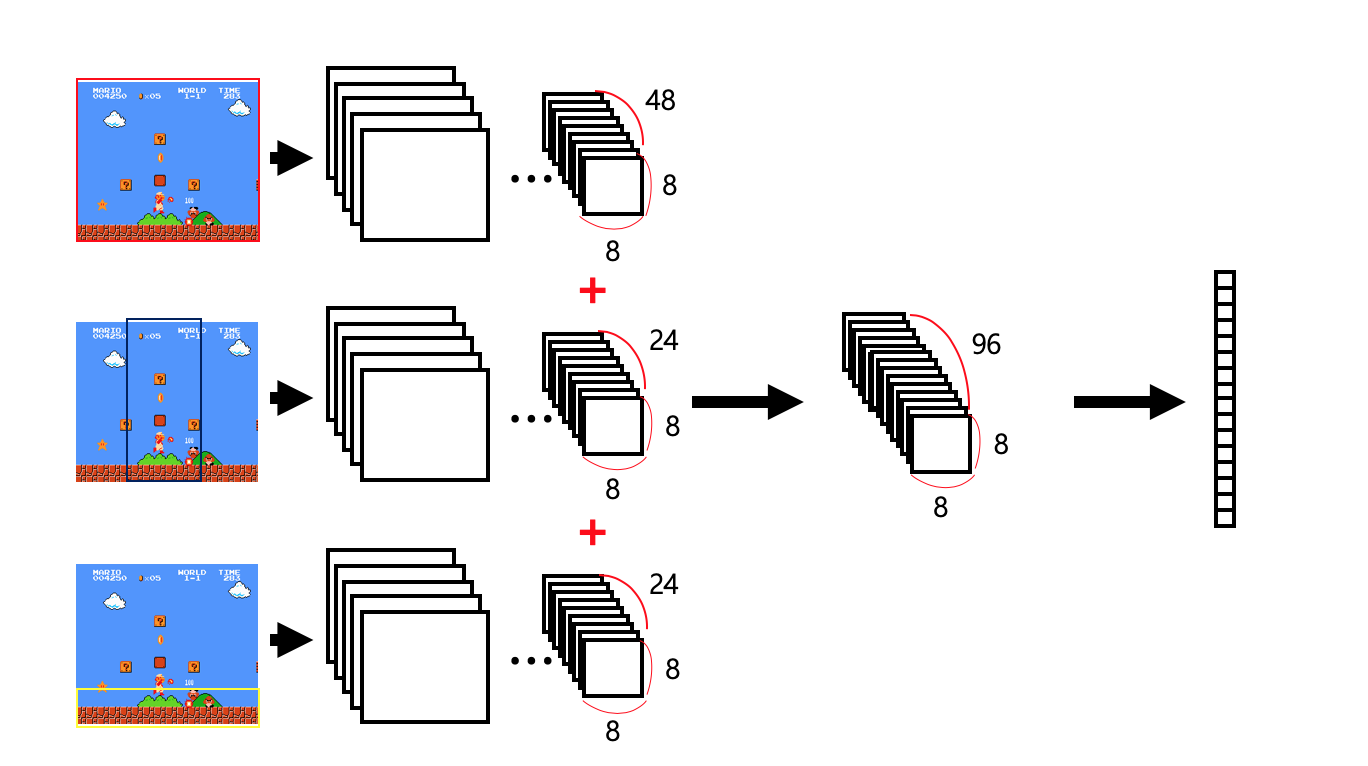
\includegraphics[width=0.8\textwidth]{FIG/split_dqn.png} \\
\end{tabular}
\caption{
	Split DQN의 CNN 처리 방식
}
\label{fig:split_dqn}
\end{center}
\end{figure}



\section{Development Settings and Plan}
\label{sec:plan}

본 절에서는 개발 환경과 프로젝트 코드에 대한 내용을 다룬다.
하위 섹션~\ref{sec:dev:gym}에서는 개발 환경 구성에 핵심이 되는 gym 라이브러리를 소개한다.
그리고 실험에 사용한 환경을 하위 섹션~\ref{sec:dev:environment}에서 소개한다.
마지막으로 하위 섹션~\ref{sec:dev:code}에서 간략히 설명한 후 프로젝트 실행 시 사용할 수 있는 옵션에 대해서 소개한다.

\subsection{OpenAI gym}
\label{sec:dev:gym}
게임을 학습하기 위해서는 입력을 통해 게임을 컨트롤하고 필요에 따라 게임을 재시작하거나 환경에 관련된 값을 얻어올 수 있는 개발환경이 필요하다.
슈퍼 마리오 브라더스의 경우 다양한 NES 에뮬레이터로 PC환경에서 게임을 실행시킬 수 있다.
OpenAI에서는 다양한 게임에 대해 강화학습을 적용할 수 있도록 gym 라이브러리를 제공하였는데, 슈퍼 마리오 브라더스의 에뮬레이터 환경과 gym 라이브러리를 연동한 것이 바로 gym-super-mario-bros~\cite{GYMMario} 이다.
이를 활용하면 게임 화면 이외의 게임내의 추가 정보를 메모리 영역으로부터 읽어와서 Table~\ref{tab:mario:info}와 같은 정보를 매 상황마다 얻어올 수 있다.

\begin{table}[h]
\centering
	\caption {
		게임 화면외 얻을 수 있는 추가 정보. 매 action을 입력할 때 마다 다음 화면 정보와 함께 얻어올 수 있다.
	}
	\label{tab:mario:info}
\begin{tabular}{ll}
\toprule
추가 정보      & \multicolumn{1}{c}{설명} \\
\midrule
Distance       & 출발점에서부터의 거리 \\
Life           & 마리오의 잔여 생명 \\
Score          & 현재 점수 \\
Coins          & 현재까지 획득한 코인의 수 \\
Time           & stage를 완료해야하는 제한 시간 \\
Player status  & 마리오의 변신 정도 \\
Ignore         & 마리오가 갇혀있는 상태 \\
\bottomrule
\end{tabular}
\end{table}

우리는 python 기반의 NES 에뮬레이터와 gym 환경을 사용하므로 python이 구동가능한 환경이면 우리 모델을 학습시킬 수 있다.
우리 모델을 학습시킬 때 GPU 가속을 통해 연산 효율을 최적화 하기 위해서 CUDA 환경이 설치된 ubuntu 16.04 에서 모델을 학습시키도록 하였다.
특히 학습시에는 게임을 렌더링하지 않도록 하여 최대한 빠른 시간에 많은 에피소드를 학습할 수 있도록 한다.

\subsection{Test Envirnment}
\label{sec:dev:environment}
우리 프로젝트의 코드는 python으로 작성되었으며 GPU가속을 통한 학습을 위해 tensorflow 라이브러리를 사용하였다.
실험에 사용한 컴퓨터는 다음과 같은 사양을 가지고 있다.
\begin{itemize}
	\item \textbf{CPU}:
		Intel Xeon E5-2630 v4 2.2GHz, 25M cache
	\item \textbf{Memory}:
		500GB, 2133MHz
	\item \textbf{GPU}:
		NVIDIA GTX 1080ti 4개
\end{itemize}
모델별로 각각의 실험 세팅에 따라 하나의 GPU를 할당하였으며 효율적인 연산을 위해 GPU 하나당 한번에 5개의 실험을 수행하여 CPU, GPU 자원을 거의 모두 활용하도록 하였다.
실험 도중에 메모리는 비교적 여유있는 편이었다.

\subsection{Code Structure}
\label{sec:dev:code}
실험에 사용한 코드는 최대한 중복 코드를 피하여 여러 가지 모델을 쉽게 테스트할 수 있도록 설계되었다.
소스코드의 구조는 아래와 같다.
%
\begin{itemize}
	\item \textbf{main.py}:
		모델의 train/test의 골격이 되는 구조를 가지고 있다. gym을 통해 마리오 게임을 로드하고 argument에 따라 선택된 모델을 불러와 train이나 test를 수행한다.
	\item \textbf{ReplayMemory.py}:
		DQN의 핵심이 되는 replay memory를 구현하고 있다.
		각각의 행동을 (state, action, reward, next state, done) tuple로 저장하고 있으며 이를 나중에 학습에 활용하게 된다.
	\item \textbf{DQN.py}:
		\dqn 모델의 tensorflow graph를 구성하는 코드이다.
		모델의 생성 및 추론, 학습, 파일로 저장, 불러오기를 수행할 수 있다.
	\item \textbf{SplitDQN.py}:
		\sdqn 모델의 tensorflow graph를 구성하는 코드이다.
		모델에 대한 지원하는 기능은 DQN.py와 같다.
	\item \textbf{SADQN.py}:
		\sadqn 모델의 tensorflow graph를 구성하는 코드이다.
		모델에 대한 지원하는 기능은 DQN.py와 같다.
	\item \textbf{SADQNp.py}:
		\sapdqn 모델의 tensorflow graph를 구성하는 코드이다.
		모델에 대한 지원하는 기능은 DQN.py와 같다.
\end{itemize}
%
위와 같이 모델의 코드를 분리해 놓음으로써 다양한 모델이 그 외 환경에 대한 코드를 공유하여 사용하는 구조이다.
main.py를 실행할 때 hyper parameter와 모델의 선택에 대한 값들을 인자로 받을 수 있는 데 상세 사항은 아래와 같다.
%
\begin{itemize}
	\item \textbf{--replay\_memory\_total}:
		Replay memory에서 최대 몇개의 동작을 저장할 지 지정.
		기본값은 50,000.
	\item \textbf{--training\_batch\_size}:
		모델의 학습시 batch의 크기.
		기본값은 16.
	\item \textbf{--gamma}:
		모델의 loss값을 계산할 때, 한 step 다음 state에서 얻을 수 있는 q 기대값에 대한 decay factor.
		기본값은 0.8.
	\item \textbf{--learning\_rate}:
		Gradient descent 를 통해 모델을 학습할 때, adam optimizer의 learning rate.
		기본값은 1e-3.
	\item \textbf{--epsilon}:
		e-greedy 방법을 통해 매 step시 임의의 action을 선택하게 되는 데, 이 경우의 확률값.
		기본값은 0.02.
	\item \textbf{--max\_steps}:
		Train 시 에피소드를 계속 반복하여 학습하게 되는 데, 이때 에피소드들을 통틀어 학습에 사용하는 최대 step의 값.
		기본값은 1000000.
	\item \textbf{--model\_name}:
		사용할 모델의 이름. DQN, SDQN, SADQN, SAPDQN 중 하나의 값을 가져야 한다.
		기본값은 DQN.
	\item \textbf{--play\_mode}:
		이 옵션은 boolean 타입의 값이며 선언될 경우 학습을 하지 않고 render를 포함에 게임을 플레이 한다.
		기본값은 false.
	\item \textbf{--reward\_mode}:
		서로 다른 reward 함수 중 하나를 선택한다. R0, R1, R2 중 하나의 값을 가져야 한다.
		기본값은 R0.
\end{itemize}
%

%\subsection{개발 일정}
%\label{sec:dev:schedule}
%본 프로젝트는 두 사람이 협동하여 4, 5월간 9주에 걸쳐서 수행한다.
%프로젝트 전반부에는 작업의 효율을 위해 개발환경 세팅 및 기존 방법을 구현할 사람과 새로운 방법을 연구할 사람으로 나누어 분업한다.
%Table~\ref{tab:schedule}은 프로젝트 구성원이 각 역활을 수행할 일정을 나타낸다.
%5주차까지 개발환경 세팅과 기존 방법으로 학습해보는 것까지 완료한 후 서로 공유하여 각자 개발환경을 갖출 수 있도록 한다.
%이 후 새로운 방법을 연구한 것을 공유하여 제안 메소드를 협업하여 구현한 후 학습시킨다.
%
%% Please add the following required packages to your document preamble:
%% \usepackage{multirow}
%\begin{table}[]
%\centering
%	\caption {
%		개발 일정.
%		크게 개발환경 설정 및 기존 방법으로 게임을 학습하는 담당과 새로운 방법을 연구 하는 담당으로 나뉜다.
%		이후 개발환경을 공유한 뒤, 새로운 방법 개발에 협력한다.
%	}
%	\label{tab:schedule}
%\begin{tabular}{clccccccccc}
%\toprule
%                     & \multicolumn{1}{c}{} & \multicolumn{4}{c}{4월} & \multicolumn{5}{c}{5월} \\
%                     & \multicolumn{1}{c}{} & 1    & 2   & 3   & 4   & 1  & 2  & 3  & 4  & 5  \\
%\midrule
%\multirow{3}{*}{구본헌} & 개발환경 세팅              & *    & *   & *   &     &    &    &    &    &    \\
%                     & 기존 방법으로 학습           &      &     & *   & *   & *  &    &    &    &    \\
%                     & 제안 방법 개발             &      &     &     &     &    & *  & *  & *  & *  \\
%\midrule
%\multirow{3}{*}{김정훈} & 개발환경 세팅              &      &     & *   &     &    &    &    &    &    \\
%                     & 새로운 방법 연구           & *    & *   & *   & *   & *  &    &    &    &    \\
%                     & 제안 방법 개발             &      &     &     &     &    & *  & *  & *  & * \\
%\bottomrule
%\end{tabular}
%\end{table}
%
%신경학습망을 통한 모델의 특성상, 하이퍼 파라미터의 세팅에 따라 성능의 변화가 클 가능성이 높다.
%프로젝트 구성원은 각자 가지고 있는 컴퓨팅 환경을 최대한 활용하여 하이퍼 파라미터 세팅을 분배하여 각자 학습하며, 주기적으로 서로의 결과물을 비교하여 더 나은 세팅을 찾도록 한다.
%


\section{Experiments}
\label{sec:experiments}

\subsection{Evaluation}
\label{sec:exp:evaluation}
Table~\ref{tab:evaluation}에서 보이는 바와 같이 \sdqnname를 사용한 모델에서 마리오가 가장 먼 거리를 이동하였다.
우리의 학습 목표가 빠른 시간내에 스테이지를 감안하면 모델의 성능 평가에 시간적인 요소가 들어가야 한다.
하지만 스테이지를 클리어하지 못한 상황에서는 시간이 많이 걸리더라도 먼 거리를 이동하는 것이 바람직하다.
아쉽게도 본 실험에 사용한 모델들 (\dqnname, \sdqnname, \sadqnname) 모두 월드 1-1을 클리어하는 데까지 학습되지 못하였다.
본 실험 시간이 충분하지 못하여 각 모델들은 동일하게 10시간 동안의 학습시키고, 학습하는 중간에 마리오의 생명을 모두 소진한 경우 테스트 모드로 변환하여 마리오의 이동거리를 측정하였다.
테스트 모드에서는 학습때와는 달리 e-greedy 방법을 사용하지 않고 모델의 q-network을 사용하여 매 action을 기대되는 q값을 최대화 하도록 선택하였다.
이와 같은 실험에서 화면 분활을 통해 특정 부분에 대해 집중적으로 feature를 수집하는 \sdqnname이 마리오를 가장 먼거리로 이동시켰다.

\begin{table}[h]
\centering
\caption {
	모델별 마리오 도달거리. 월드 1-1에서만 테스트하였으며 많은 거리를 이동할 수록 숫자가 크다.
}
\label{tab:evaluation}
\begin{tabular}{llll}
\toprule
     & \dqnname  & \sdqnname & \sadqnname \\
\midrule
도달거리 & 1641 & 1784  & 1675  \\
\bottomrule
\end{tabular}
\end{table}

우리의 기대와는 달리, \sdqnname에서 attention network를 추가한 \sadqnname의 성능이 낮게 평가되었다.
이는 충분한 학습시간을 가지지 못한 우리의 상황이 학습하여야하는 파라미터의 수가 많은 \sadqnname에게 불리한 요소로 작용되었을 것으로 추측된다.


\subsection{Effectiveness of Dropout and Batch Normalization}
\label{sec:exp:dropout}
일반적인 neural network에서 dropout과 batch normalization은 모델의 overfitting을 막기위해 널리 사용되는 방법이다.
DQN기반의 모델들도 q-value function을 neural network에 기반한 함수를 사용하고 있으므로 해당 기법들이 모델의 학습에 도움이 될 것이라고 생각하였다.
\sapdqnname은 \sadqnname에서 각 CNN의 앞단에 batch normalization layer를 추가하고, action의 q값을 추론하기 직전의 MLP (Multi Layer Perceptron) 직후 30\%의 노드를 dropout시키는 dropout layer를 추가하였다.
결과적으로 \sapdqnname은 학습되는 데 실패하여 마리오의 이동거리가 40을 채 넘지 못하였다.

\begin{figure}[h]
\centering
	\begin{subfigure}[]{.48\textwidth}
		\centering
		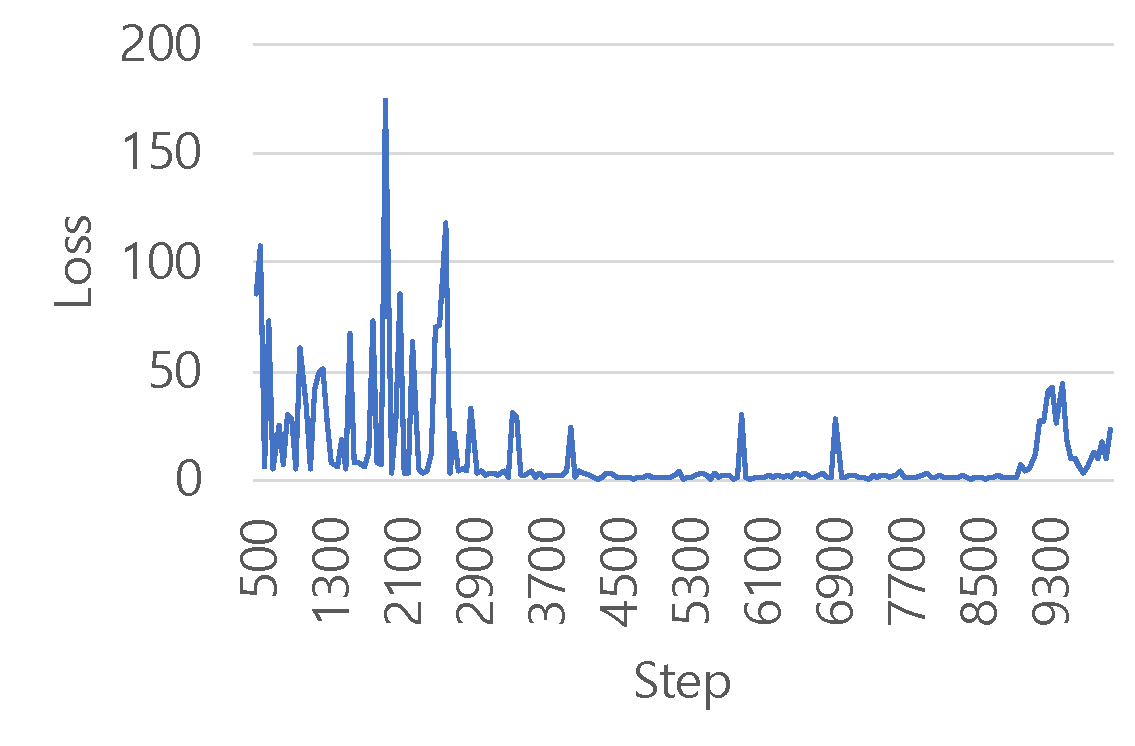
\includegraphics[width=1.\textwidth]{FIG/Loss_SADQN.pdf}
		\caption{Loss of \sadqnname}
		\label{fig:loss_sadqn}
	\end{subfigure}%
	\begin{subfigure}[]{.48\textwidth}
		\centering
		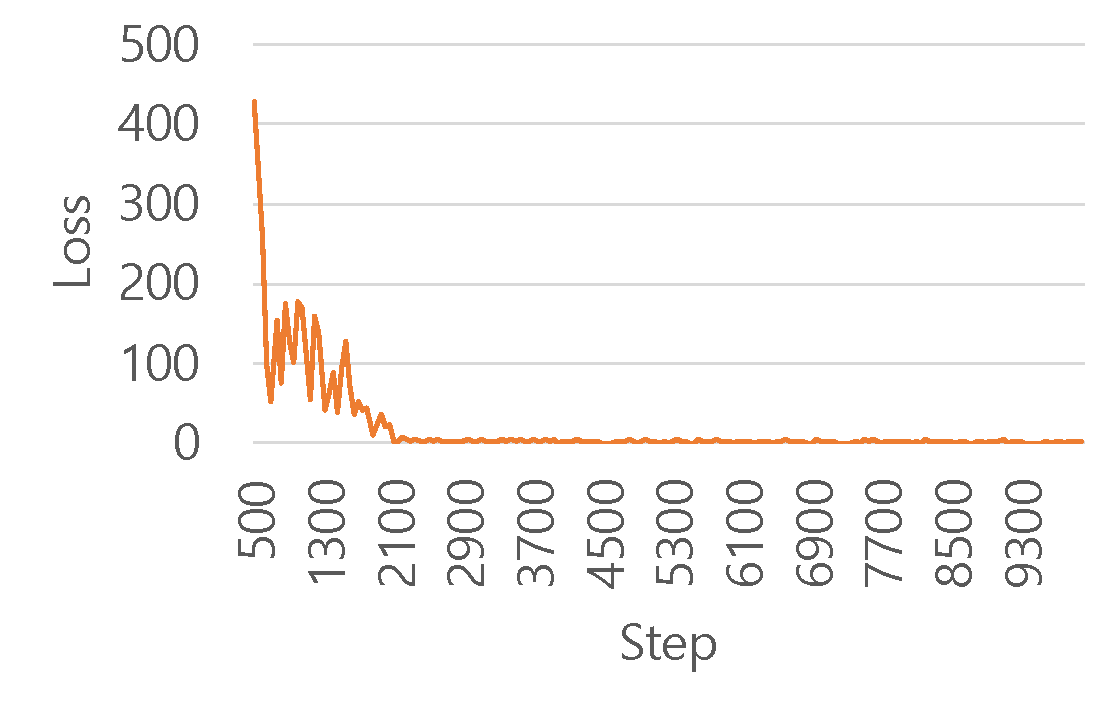
\includegraphics[width=1.\textwidth]{FIG/Loss_SAPDQN.pdf}
		\caption{Loss of \sapdqnname}
		\label{fig:loss_sapdqn}
	\end{subfigure}%
\caption{
	Step별 loss의 변화. 결과적으로 더 멀리 마리오를 이동시킨 \sadqnname의 경우 지속적으로 loss가 상승하였다가 감소하는 구간이 확인된다.
}
\label{fig:loss}
\end{figure}

Figure~\ref{fig:loss}는 step별로 \sadqnname과 \sapdqnname의 loss가 어떻게 변화하는지 보여주고 있다.
\sadqnname는 지속적으로 loss가 상승하였다가 감소하는 구간이 확인되는 반면, \sapdqnname은 loss가 한번 감소된 이후 그것을 유지하고 있다.
\sadqnname의 경우, 마리오가 더 멀리 나아가서 새로운 state를 발견하였을 때, 미지의 구간에 대한 q값 때문에 loss가 상승하였다가 이에 대한 학습이 끝나면 loss가 감소하는 것을 반복하고 있다.
반면, \sapdqnname은 마리오가 계속 시작지점에만 머물러 있기 때문에 새로운 state를 발견하지 못하고 있다.
따라서 지속적으로 발전해나가는 모델의 loss의 변화는 Figure~\ref{fig:loss_sadqn}과 같은 모양을 가지게 된다.

\subsection{Reward}
\label{sec:exp:reward}
% 이건 그냥 써본건데 혹시라도 각각의 리워드 세팅에 따라 실험한게 있다면 결과를 쓰기 위해 놔둬봤어영
Reward는 강화학습에서 모델 학습의 성공 여부를 결정짓는 중요한 요소이다.
Reward를 계산할 때 우리는 3가지 요소를 고려하였다.
첫번째 요소는 마리오의 가로 방향 이동거리인데, 좌측으로 이동할 수록 reward가 증가하고 우측으로 이동할 수록 감소한다.
두번째 요소는 마리오의 이동이 없었을 때의 패널티이다.
이때 reward를 0으로 주거나 감소시키기도 하였다.
마지막 요소는 게임의 남은 시간 (초) 이다. 남은 시간이 줄어들 수록 reward를 감소시켰다.
우리는 본 실험에서 3가지의 서로 다른 Reward를 구현하고 이전에 성능이 제일 잘 나왔던 \sadqnname으로 테스트 하였다.
3가지 Reward 세팅은 다음과 같다.
\begin{itemize}
	\item \textsc{R0}:
		가로 방향 +10 이동시 reward 5 증가 및 -10 이동시 5 감소. 이동이 없을때 패널티는 없으나, 남은 시간이 1 줄어들때 마다 reward 1 감소.
	\item \textsc{R1}:
		가로 방향 +3 이동시 reward 5 증가 및 -3 이동시 5 감소. 이동이 없을때 reward 1 감소 및 남은 시간이 1 줄어들때 마다 reward 1 감소.
	\item \textsc{R2}:
		가로 방향 +1 이동시 reward 5 증가 및 -1 이동시 5 감소. 이동이 없을때 reward 1 감소 및 남은 시간이 1 줄어들때 마다 reward 1 감소.
\end{itemize}

\begin{table}[h]
\centering
\caption {
	Reward별 \sdqnname의 마리오 도달거리.
}
\label{tab:reward}
\begin{tabular}{llll}
\toprule
     & R0  & R1 & R2 \\
\midrule
도달거리 & 1423 & 1784  & 1439  \\
\bottomrule
\end{tabular}
\end{table}

Table~\ref{tab:reward}에서 각 reward별 \sadqnname의 마리오 도달거리를 확인할 수 있다.
R1이 가장 좋은 성능을 보이고 있다.
R0의 경우에는 이동이 없을 때 패널티가 없어서 마리오가 계속 멈추는 현상이 일어났다.
이때 모델은 q값을 0으로 추측하게 되는데 이는 모델 내부의 parameter값들을 0으로 수렴시켜서 결과적으로 loss의 값도 크게 감소하지만 마리오가 계속해서 아무 행동을 하지않게 하는 악순환을 반복하고 있다.
R2의 경우 이동에 대한 reward가 너무 민감하기 때문에 reward의 값이 너무 커져서 모델에게 혼동을 주는 것으로 보인다.
R1은 이동이 없을 때 reward를 감소시켜 마리오가 이동할 수 있도록 자극을 주며, 가로 방향으로의 이동에 대해서도 적절한 reward를 주어 \sadqnname의 학습을 돕는다.

%첫 번째로는 마리오가 과거 위치보다 좌측으로 10만큼 이동하였다면 이는 목적지에서 더욱 멀어지는 방향으로 가고 있다 판단되어 -5만큼의 reward를 제공한다. 
%만약 마리오가 과거 위치보다 우측으로 10만큼을 이동한다면 이는 목적지와 더 가까워지고 있다는 의미로 +5만큼의 reward를 제공한다. 
%두 번째로 시도한 방식은 첫 번째 방식에서 이동 폭을 10에서 3으로 감소시켰다.
%또한 만약 마리오가 이전 위치와 비교하였을 때 아무런 변화가 없다면 -1만큼의 reward를 제공함으로써 마리오를 움직이게 한다.
%마지막 세 번째 방식은 두 번째 방식에서 이동 폭을 3에서 1로 감소시켰다.


\section{Conclusion}
\label{sec:conclusion}
%지금까지 우리는 본 프로젝트에서 진행했던 내용에 대해 살펴보았다.
%해당 프로젝트를 진행하면서 굉장히 많은 어려움이 존재했다. 
%모델을 다양한 방식으로 수정하고 추가 작업을 진행하여도 성능이 좀처럼 향상되지 않았다.
%따라서 프로젝트 초반에 목표로 정했던 가능한 빠른 시간안에 완주하는 것은 정말 쉽지 않았고, 완주를 하는 것조차 굉장히 어려운 문제였다는 것을 깨달았다.
%
%비록 프로젝트 초반에 설정했던 목표는 달성하지 못했지만 슈퍼 마리오 브라더스 게임을 통해 강화학습을 실제로 구현하고 구현에 필요한 기법들을 서베이하며 강화학습에 대해 많은 것들을 배울 수 있는 기회가 되었다.

본 프로젝트에서 우리는 슈퍼 마리오 브라더스 게임을 DQN 기반의 강화학습 모델로 play할 수 있는 프로그램을 개발 하였다.
기존 아타리 게임등에서 좋은 성능을 보인다고 알려진 DQN을 기반으로 마리오 게임을 좀 더 잘 이해할 수 있도록 화면을 나눠서 feature를 추출하는 \sdqnname을 제안하였고, 더 나아가 attention network를 추가한 \sadqnname을 통해 성능 향상을 도모하였다.
하지만 강화 학습의 특징인 수 많은 hyper parameter들 (CNN 네트워크 구성, replay memory 관련 parameter, optimizer 관련 parameter, 그리고 reward 함수)과 긴 학습시간으로 인해 최적의 세팅과 결과를 얻어내는 데에는 부족한 점이 있었다.
때문에 프로젝트 초반에 설정하였던 목표인 사람보다 빠른 시간내에 완주는 달성하지 못하였다.
하지만 사람의 동작에 따른 intuition인 화면 분할이나 일부 부분에 집중하는 방법을 통해서 일반적인 DQN보다 높은 성능을 얻을 수 있었다는 점은 고무적이었다.



%\newpage
%\balance
\bibliographystyle{plain}
\bibliography{paper}

\end{document}

